\documentclass[a4paper,10pt,DIV=14]{article}
\usepackage{graphicx}
\usepackage[utf8]{inputenc} % korrekte Darstellung von Umlauten u. Sonderzeichen
\usepackage[ngerman]{babel} % Sprachpaket, ngerman = neue deutsche Rechtschreibung
\usepackage{amsmath} % Setzen mathematischer Formeln
\usepackage{amsfonts} %mathbb
\usepackage{titlesec}
\usepackage{float}
\usepackage{caption}
\usepackage{fancyvrb}
\usepackage{siunitx}
\usepackage{booktabs}
\usepackage{enumitem}
\usepackage{tikz}
\usetikzlibrary{positioning}
\usetikzlibrary{matrix}

\usepackage{subcaption}


\usepackage{tikz}
\usetikzlibrary{3d}
\usetikzlibrary{shadings}
\definecolor{mypurple}{RGB}{255,0,255}

\makeatletter
\tikzoption{canvas is xy plane at z}[]%
{   \def\tikz@plane@origin{\pgfpointxyz{0}{0}{#1}}%
	\def\tikz@plane@x{\pgfpointxyz{1}{0}{#1}}%
	\def\tikz@plane@y{\pgfpointxyz{0}{1}{#1}}%
	\tikz@canvas@is@plane
}
\makeatother 

\usepackage{tabularx}
\newcolumntype{L}[1]{>{\raggedright\arraybackslash}p{#1}} % linksbündig mit Breitenangabe
\newcolumntype{C}[1]{>{\centering\arraybackslash}p{#1}} % zentriert mit Breitenangabe
\newcolumntype{R}[1]{>{\raggedleft\arraybackslash}p{#1}} % rechtsbündig mit Breitenangabe

\newcommand{\gqq}[1]{\glqq{}#1\grqq{}}
\newcommand{\gq}[1]{\glq{}#1\grq{}}
\newcommand{\dg}[1]{#1^\circ}

\renewcommand{\thesection}{Aufgabe \arabic{section}:}
\renewcommand{\thesubsection}{\alph{subsection})}
\renewcommand{\thesubsubsection}{\roman{subsubsection}}

\titleformat{\subsection}
{\normalsize}{\thesubsection}{1em}{}


\captionsetup[figure]{labelformat=empty}

\begin{document}

\title{Graphische Datenverarbeitung WS17/18 \\ Theorieübung 4}
\author{
  Salmah Ahmad (2880011)
  \and
  Markus Höhn (1683303)
  \and
  Tobias Mertz (2274355)
  \and
  Steven Lamarr Reynolds (1620638)
  \and
  Sascha Zenglein (2487032)
}

\maketitle

\section{Beleuchtung (4 Punkte)}

\subsection{(1 Punkt)}

\subsubsection{}

Umrechnung von RGB in HSV: \\
\newline
$
R' = R/255\\
G' = G/255\\
B' = B/255\\
max = max((R', G', B'))\\
min = min((R', G', B'))\\
\Delta = max - min
$\\~\\
$t di
H = \begin{cases}
0^\circ &\Delta = 0\\
60^\circ \times (\frac{G'-B'}{\Delta}) &, max = R'\\
60^\circ \times (\frac{B'-R'}{\Delta}+2) &, max = G'\\
60^\circ \times (\frac{R'-G'}{\Delta}+4) &, max = B'\\
\end{cases}
$\\~\\~\\
$
S = \begin{cases}
0 & max = 0\\
\frac{\Delta}{max}, &max \neq 0\\
\end{cases}
$\\~\\~\\
$
V = max
$\\

$
\text{Grün}_{HSV} = (120^\circ, 1, 1)
$\\
$
\text{Magenta}_{HSV} = (300^\circ, 1, 1)
$

\subsubsection{}

$
f_{RGB}(x) = ((1-x)\cdot255, \ x\cdot255, \ (1-x)\cdot255)
$\\
$
f_{HSV} = ((1-x)\cdot300^\circ + x\cdot 120^\circ, \ 1, \ 1)
$

\subsubsection{}

RGB Cube:\\

\pgfmathtruncatemacro{\Divisions}{30}
\pgfmathsetmacro{\Cube}{3}

\begin{tikzpicture}
[   x={(0.5cm,0.5cm)},
y={(0.95cm,-0.25cm)},
z={(0cm,0.9cm)}
]
\begin{scope}[canvas is yz plane at x=-\Cube/2] %front
\shade[lower right=mypurple, lower left=blue, upper right=white, upper left=cyan] (-1,-1) rectangle (1,1);
\clip (-\Cube/2,-\Cube/2) rectangle (\Cube/2,\Cube/2);
\colorlet{BL}[RGB]{blue}
\colorlet{BR}[RGB]{mypurple}
\colorlet{TL}[RGB]{cyan}
\colorlet{TR}[RGB]{white}
\foreach \x in {1,...,\Divisions}
{   \pgfmathtruncatemacro{\px}{(\x-1)/(\Divisions-1)*100}
	\colorlet{B}[RGB]{BR!\px!BL}
	\colorlet{T}[RGB]{TR!\px!TL}
	\foreach \y in {1,...,\Divisions}
	{   \pgfmathtruncatemacro{\py}{(\y-1)/(\Divisions-1)*100}
		\fill[T!\py!B] ({-\Cube/2+\Cube*(\x-1)/\Divisions},{-\Cube/2+\Cube*(\y-1)/\Divisions}) rectangle ({-\Cube/2+\Cube*(\x+0.1)/\Divisions},{-\Cube/2+\Cube*(\y+0.1)/\Divisions});
	}
}
\draw (-\Cube/2,-\Cube/2) rectangle (\Cube/2,\Cube/2);
\end{scope}

\begin{scope}[canvas is xz plane at y=\Cube/2] %right
\clip (-\Cube/2,-\Cube/2) rectangle (\Cube/2,\Cube/2);
\colorlet{BL}[RGB]{mypurple}
\colorlet{BR}[RGB]{red}
\colorlet{TL}[RGB]{white}
\colorlet{TR}[RGB]{yellow}
\foreach \x in {1,...,\Divisions}
{   \pgfmathtruncatemacro{\px}{(\x-1)/(\Divisions-1)*100}
	\colorlet{B}[RGB]{BR!\px!BL}
	\colorlet{T}[RGB]{TR!\px!TL}
	\foreach \y in {1,...,\Divisions}
	{   \pgfmathtruncatemacro{\py}{(\y-1)/(\Divisions-1)*100}
		\fill[T!\py!B] ({-\Cube/2+\Cube*(\x-1)/\Divisions},{-\Cube/2+\Cube*(\y-1)/\Divisions}) rectangle ({-\Cube/2+\Cube*(\x+0.1)/\Divisions},{-\Cube/2+\Cube*(\y+0.1)/\Divisions});
	}
}
\draw (-\Cube/2,-\Cube/2) rectangle (\Cube/2,\Cube/2);
\end{scope}

\begin{scope}[canvas is xy plane at z=\Cube/2] %top
\clip (-\Cube/2,-\Cube/2) rectangle (\Cube/2,\Cube/2);
\colorlet{BL}[RGB]{cyan}
\colorlet{BR}[RGB]{green}
\colorlet{TL}[RGB]{white}
\colorlet{TR}[RGB]{yellow}
\foreach \x in {1,...,\Divisions}
{   \pgfmathtruncatemacro{\px}{(\x-1)/(\Divisions-1)*100}
	\colorlet{B}[RGB]{BR!\px!BL}
	\colorlet{T}[RGB]{TR!\px!TL}
	\foreach \y in {1,...,\Divisions}
	{   \pgfmathtruncatemacro{\py}{(\y-1)/(\Divisions-1)*100}
		\fill[T!\py!B] ({-\Cube/2+\Cube*(\x-1)/\Divisions},{-\Cube/2+\Cube*(\y-1)/\Divisions}) rectangle ({-\Cube/2+\Cube*(\x+0.1)/\Divisions},{-\Cube/2+\Cube*(\y+0.1)/\Divisions});
	}
}
\draw (-\Cube/2,-\Cube/2) rectangle (\Cube/2,\Cube/2);
\end{scope}
\draw [-stealth](-\Cube/2,\Cube/2, -\Cube/2) -> (\Cube/2,-\Cube/2, \Cube/2);
\end{tikzpicture}\\


HSV Cone: \\
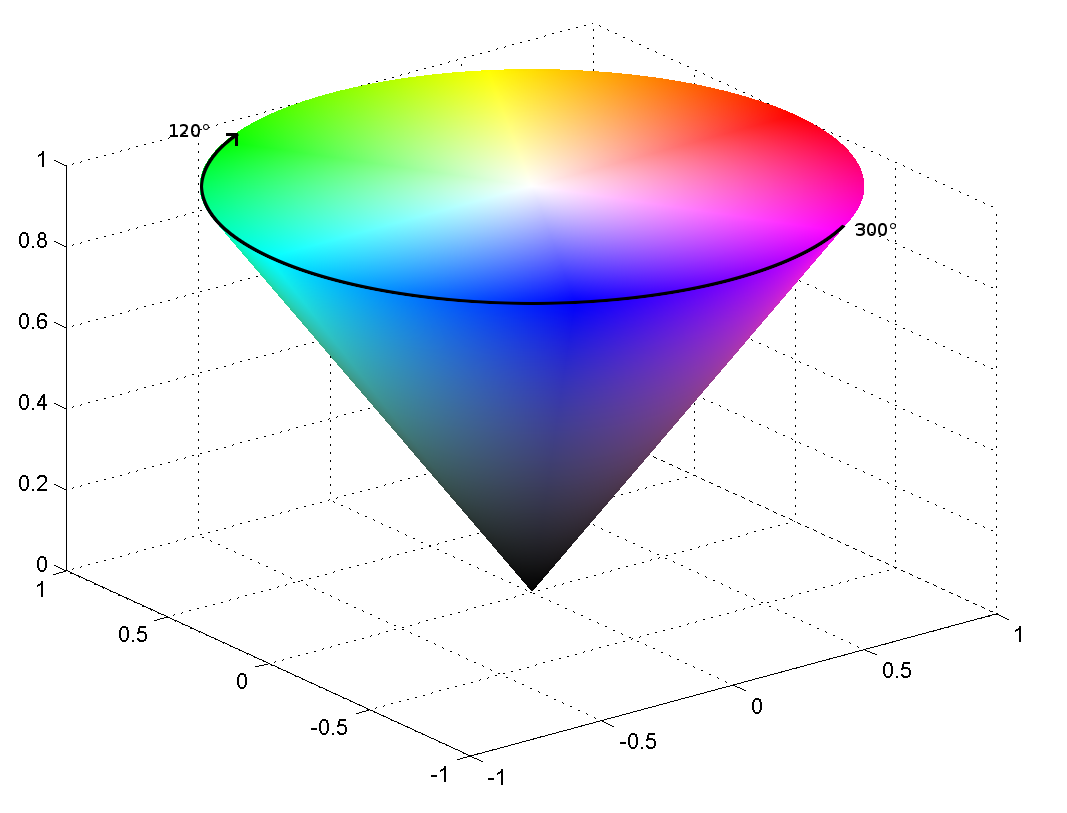
\includegraphics[scale=0.5]{hsv}

\subsubsection{}

\definecolor{rgb1}{RGB}{204, 51, 204}
\definecolor{rgb2}{RGB}{153, 102, 153}
\definecolor{rgb3}{RGB}{128, 128, 128}
\definecolor{rgb4}{RGB}{102, 153, 102}
\definecolor{rgb5}{RGB}{51, 204, 51}

\definecolor{hsv1}{RGB}{102, 0, 255}
\definecolor{hsv2}{RGB}{0, 51, 255}
\definecolor{hsv3}{RGB}{0, 128, 255}
\definecolor{hsv4}{RGB}{0, 204, 255}
\definecolor{hsv5}{RGB}{0, 255, 153}

$
x_1 = 0.2\\
x_2 = 0.4\\
x_3 = 0.5\\
x_4 = 0.6\\
x_5 = 0.8\\~\\
f_{RGB}(x_1) = (204, 51, 204)\tikz \fill [rgb1] (0.1,0.1) rectangle (0.4,0.4);\\
f_{RGB}(x_2) = (153, 102, 153)\tikz \fill [rgb2] (0.1,0.1) rectangle (0.4,0.4);\\
f_{RGB}(x_3) = (127.5, 127.5, 127.5)\tikz \fill [rgb3] (0.1,0.1) rectangle (0.4,0.4);\\
f_{RGB}(x_4) = (102, 153, 102)\tikz \fill [rgb4] (0.1,0.1) rectangle (0.4,0.4);\\
f_{RGB}(x_5) = (51, 204, 51)\tikz \fill [rgb5] (0.1,0.1) rectangle (0.4,0.4);\\~\\
f_{HSV}(x_1) = (264^\circ, 1, 1)\tikz \fill [hsv1] (0.1,0.1) rectangle (0.4,0.4);\\
f_{HSV}(x_2) = (228^\circ, 1, 1)\tikz \fill [hsv2] (0.1,0.1) rectangle (0.4,0.4);\\
f_{HSV}(x_3) = (210^\circ, 1, 1)\tikz \fill [hsv3] (0.1,0.1) rectangle (0.4,0.4);\\
f_{HSV}(x_4) = (192^\circ, 1, 1)\tikz \fill [hsv4] (0.1,0.1) rectangle (0.4,0.4);\\
f_{HSV}(x_5) = (156^\circ, 1, 1)\tikz \fill [hsv5] (0.1,0.1) rectangle (0.4,0.4);\\~\\
$
Der Farbverlauf im RGB-Cube geht von der unteren rechten pinken Ecke durch den Cube zu der oberen linken grünen Ecke. Dadurch entsteht ein Farbverlauf durch den Grauwert RGB(127.5, 127.5, 127.5). Die Rot-, Grün- und Blauwerte verändern sich entsprechend des Eingabewertes.\\
Im HSV-Raum bleiben Saturation und Value konstant, während der Hue-Wert sich ändert. So entsteht ein Farbverlauf von pink bei Hue=300$^\circ$ über die Blauwerte des Cones bis zu grün bei Hue=120$^\circ$. 

\subsection{(1 Punkt)}%b

\textbf{Isotropic BRDF}

Ist invariant bezüglich Rotation um die Normale. Kann vielleicht local berrechnet werden?
Das Isotropische Material (z.B Plastik)


\textbf{BRDF}

Reflexioneigenschaften sind unabähngig von der Position. Daher kann BRDF local berrechnet werden.
Das Homogene Material (z.B gebürstetes Metall) kann auch local berrechnet werden.

\textbf{Spatially Varying BRDF}

Verwendet eine 2d Location über dem Object Surface. Kann daher local berrechnet werden.

\textbf{BSSRDF}

Licht verlässt die Oberfläche eventuell an anderer Stelle. Daher kann es nicht Local berrechnet werden.
Dadurch kann Licht von durchlässigen Materialien an andere abgegeben werden.
Dadurch kann kein Material mehr local berrechnet werden.

\textbf{Scattering Function}

Abhängig von der Wellenlänge. Wellenlänge nicht mehr diskretisiert, Fluoreszenz. Daher nicht local berrechenbar.
Wie bei BSSRDF kann kein Material mehr Local berrechnet werden.

\textbf{allgemeines Reflexionsmodell}

Kann nicht Local berrechnet werden.
Wie bei BSSRDF kann kein Material mehr Local berrechnet werden.

% TODO: nochmal drüberlesen

\subsection{(1 Punkt)}%c
\newcommand{\VecThree}[3]{\begin{pmatrix} #1 \\ #2 \\ #3 \end{pmatrix}}
Gegeben:
\begin{gather*}
N = \VecThree{0}{1}{0}, V = \VecThree{\sqrt{0.5}}{\sqrt{0.5}}{0}, H = \VecThree{\frac{\sqrt{6}}{6}}{\frac{\sqrt{6}}{3}}{-\frac{\sqrt{6}}{6}}, \lVert L+V \rVert = \sqrt{3}, k = 1, I_{BP} = \frac{\sqrt{6}}{3}
\end{gather*}
\\
\begin{align*}
I_p &= f_p(\gamma) = (R(L)^T \cdot V)^k \cdot E = cos^k(\gamma) \cdot E \\
I_{BP} &= f_{BP}(\phi) = (H^T \cdot N)^k \cdot E = cos^k(\phi) \cdot E = \frac{\sqrt{6}}{3}\\
\phi &= \arccos(H^T \cdot N) = \arccos\left(\frac{\sqrt{6}}{3}\right) \approx 0.615\\~\\
E &= \frac{\frac{\sqrt{6}}{3}}{(H^T \cdot N)^k} = \frac{\sqrt{6} \cdot (H^T \cdot N)^k}{3} \\
&= \frac{\sqrt{6} \cdot \left(\VecThree{\frac{\sqrt{6}}{6}}{\frac{\sqrt{6}}{3}}{-\frac{\sqrt{6}}{6}}^T \cdot \VecThree{0}{1}{0}\right)^1}{3} = \frac{\sqrt{6} \cdot \frac{\sqrt{6}}{3}}{3} =  \frac{2}{3}\\~\\
H &= \frac{L+V}{\lVert L+V \rVert} = \frac{L+V}{\sqrt{3}} \Rightarrow
\VecThree{\frac{\sqrt{6}}{6}}{\frac{\sqrt{6}}{3}}{-\frac{\sqrt{6}}{6}} = \frac{L+V}{\sqrt{3}} \\
L &= \VecThree{\frac{\sqrt{6}}{6}}{\frac{\sqrt{6}}{3}}{-\frac{\sqrt{6}}{6}} \cdot \sqrt{3} - \VecThree{\sqrt{0.5}}{\sqrt{0.5}}{0} = \VecThree{\frac{\sqrt{2}}{2}}{\sqrt{2}}{-\frac{\sqrt{2}}{2}} - \VecThree{\sqrt{0.5}}{\sqrt{0.5}}{0} = \VecThree{0}{\sqrt{0.5}}{-\frac{\sqrt{2}}{2}}\\~\\
R(L) &= - L + 2 \left(L \cdot N \right) N \\
&= - \VecThree{0}{\sqrt{0.5}}{-\frac{\sqrt{2}}{2}} + 2 \left(\VecThree{0}{\sqrt{0.5}}{-\frac{\sqrt{2}}{2}} \cdot \VecThree{0}{1}{0} \right) \VecThree{0}{1}{0} \\
&= - \VecThree{0}{\sqrt{0.5}}{-\frac{\sqrt{2}}{2}} + 2 \left( \sqrt{0.5} \right) \VecThree{0}{1}{0} \\ 
&= \VecThree{0}{\sqrt{0.5}}{\frac{\sqrt{2}}{2}}\\~\\
\gamma &= \arccos(R(L)^T \cdot V) \\
&= \arccos\left(\VecThree{0}{\sqrt{0.5}}{\frac{\sqrt{2}}{2}}^T \cdot \VecThree{\sqrt{0.5}}{\sqrt{0.5}}{0} \right) \\
&= \arccos(0.5) \approx 1.047\\~\\
I_p &= cos(\gamma) \cdot E = 0.5 \cdot E = \frac{1}{3}
\end{align*}
Lösung:
\begin{align*}
I_p &= \frac{1}{3}\\
E &= \frac{2}{3} \\
\gamma &= \arccos(0.5) \approx 1.047\\
\phi &= \arccos\left(\frac{\sqrt{6}}{3}\right) \approx 0.615 \\
L &=  \VecThree{0}{\sqrt{0.5}}{-\frac{\sqrt{2}}{2}} \\
R(L) &= \VecThree{0}{\sqrt{0.5}}{\frac{\sqrt{2}}{2}}\\
\end{align*}

\subsection{(0.5 Punkte)} %d
%TODO, auskommentiert damit niemand denkt es wäre fertig
%\begin{gather*}
%I_{BP} \neq 0 \neq I_P \\
%(R(L)^T \cdot V)^k = cos^k(\gamma) \\
%(H^T \cdot N)^k = cos^k(\phi) \\
%\gamma = \phi \\
%\Rightarrow \left\vert R(L)^T \cdot V \right\vert = \left\vert H^T \cdot N \right\vert \\
%\Rightarrow \left\vert \left(- L + 2 \left(L \cdot N \right) N\right)^T \cdot V \right\vert = \left\vert \left(\frac{L+V}{\lVert L+V \rVert}\right)^T \cdot N \right\vert
%\end{gather*}
\subsection{(0.5 Punkte)}



\clearpage
\section{Texturierung (2 Punkte)} %2

\subsection{(1 Punkt)} %2a

% Source: Vorlesung 10, Slide 13

Zu berrechnen ist die Umkehrfunktion $(u,v) = F_{\text{inv map}}(x,y,z)$.\\

Gegeben sei $u,v \in [0,1]$, $r, h$ sowie $x,y,z$.\\

Das Zylinder-Mapping gibt an:

$x = r \cdot sin(u)$

$y = v$

$z = r \cdot cos(u)$\\

Daraus ergibt sich folgende Funktionen für $v$:

\[v = \frac{y}{h}\]

Falls $x \geq 0 \Leftrightarrow u \in [0,0.5]$

\[u = \cos^{-1}(\frac{z}{\sqrt{x^2+z^2}}) \cdot \frac{1}{2\pi}\]

Sonst $x < 0 \Leftrightarrow u \in [0.5, 1]$

\[u = (2\pi - \cos^{-1}(\frac{z}{\sqrt{x^2+z^2}})) \cdot \frac{1}{2\pi}\]

Alternativ ohne Fallunterscheidung:

\[u = \frac{1}{2\pi} \cdot atan2(x,z) + 0.5\]


\subsection{(1 Punkt)} %2b

% Source: Vorlesung 10, Slide 49. Summed Area Tables

\textbf{Rechteck}\\

\begin{tikzpicture}
\draw[step=0.5cm, color=gray] (0,0) grid (2.5,2.5);
\matrix[matrix of nodes,
inner sep=0pt,
anchor=south west,
nodes={inner sep=0pt,text width=.5cm,align=center,minimum height=.5cm}]{
5 & 1 & 2 & 4 & 2 \\
2 & 3 & 4 & 1 & 1 \\
2 & 1 & 1 & 3 & 1 \\
2 & 2 & 1 & 3 & 5 \\
0 & 2 & 2 & 3 & 1 \\
};
\end{tikzpicture}

$C_{sat}$\\

\begin{tikzpicture}
\draw[step=0.5cm, color=gray] (0,0) grid (2.5,2.5);
\matrix[matrix of nodes,
inner sep=0pt,
anchor=south west,
nodes={inner sep=0pt,text width=.5cm,align=center,minimum height=.5cm}]{
 5 &  6 &  8 & 12 & 14 \\
 7 & 11 & 17 & 22 & 25 \\
 9 & 14 & 21 & 29 & 33 \\
11 & 18 & 26 & 37 & 46 \\
11 & 20 & 30 & 44 & 54 \\
};
\end{tikzpicture}

\textbf{schraffiertes Rechteck}\\

\begin{tikzpicture}
\draw[step=0.5cm, color=gray] (0,0) grid (2,1);
\matrix[matrix of nodes,
inner sep=0pt,
anchor=south west,
nodes={inner sep=0pt,text width=.5cm,align=center,minimum height=.5cm}]{
1 & 2 & 4 & 2\\
3 & 4 & 1 & 1\\
};
\end{tikzpicture}

\[c_{avg}(i_0,j_0,i_1,j_1) = \frac{\sum_{i=i_{0}}^{i_{1}} \sum_{j=j_{0}}^{j_{1}}  C[i,j]}{(i_{1}-i_{0}+1)(j_{1}-j_{0}+1)}\]

\[c_{avg}(0,1,1,4) = \frac{25 - 0 - 7 + 0}{(1-0+1)(4-1+1)} = 2.125\]

Demnach benötigen wir 2 Zugriffe (1 Zugriff für $C_{sat}[i_{1},j_{1}]$, 1 für $C_{sat}[i_{1},j_{0}-1]$) wenn man $C_{sat}$ verwendet.\\
Für die normale Berrechnung benötigen wir dagegen 8 Zugriffe (jeweils 1 Zugriff für jeden Grau-Textur-Wert).\\
Wir sparen dadurch 8 Zugriffe durch die Verwendung von $C_{sat}$.


\section{Perspektivisch korrekte Texturierung (4 Punkte)}

\subsection{(1 Punkt)}
$l_1(s) = (3, -12)^T + s(-6, 6)^T \qquad s \in [0,1]$ \\

Berechnung von p und q:\\

$l_2(t) = p + t(q-p) \qquad t \in [0,1]\\~\\
\lambda \cdot (3, -12)^T = (x_1, -4)^T\\
-12 \lambda = -4 \Rightarrow \lambda = \frac{1}{3}\\
3 \lambda = x_1 \Rightarrow x_1 = 1\\
\Rightarrow p = (1, -4)^T\\~\\
\phi \cdot (-3, -6)^T = (x_2, -4)^T\\
-6 \phi = -4 \Rightarrow \phi = \frac{2}{3}\\
-3 \phi = x_2 \Rightarrow x_2 = -2\\
\Rightarrow q = (-2, -4)^T\\~\\
l_2(t) = (1, -4) + t(-3, 0)
$\\

Bei dem Liniensegment $l_2$ werden durch die Interpolation die unterschiedlichen z-Koordinaten von P und Q vernachlässigt, wodurch die Textur möglicherweise verzerrt dargestellt wird.
\subsection{(1 Punkt)} 

$
l_3 = -4 \cdot \left( \dfrac{x_1 + s (x_2 - x_1)}{z_1 + s(z_2 - z_1)}, 1\right)^T\\
l_3 = -4 \cdot \left( \dfrac{3 - 6s}{-12 + 6s}, 1\right)^T
$

\subsection{(1 Punkt)}

$
l_2 = l_3\\
-4 \cdot \left( \frac{x_1}{x_2} + t(\frac{x_2}{z_2} - \frac{x_1}{z_1}) \right) = -4 \cdot \left( \dfrac{x_1 + s (x_2 - x_1)}{z_1 + s (z_2 - z_1)}\right)\\
-4 \cdot \left( \frac{3}{-3} + t(\frac{-3}{-6} - \frac{3}{-12}) \right) = -4 \cdot \left( \dfrac{3 - 6s }{-12 + 6s}\right)\\
\Rightarrow s = \dfrac{-12t}{-6 -6t}
$\\

Durch die Umstellung auf s können wir aus der einfachen Interpolation $l_2(t)$ die perspektivisch projezierte Interpolation $l_3(s)$ berechnen. Damit können aus den perspektivisch verzerrten Texturkoordinaten die perspektivisch korrekten Koordinaten errechnet werden. 

\subsection{(1 Punkt)}

ohne perspektivische Korrektur:\\
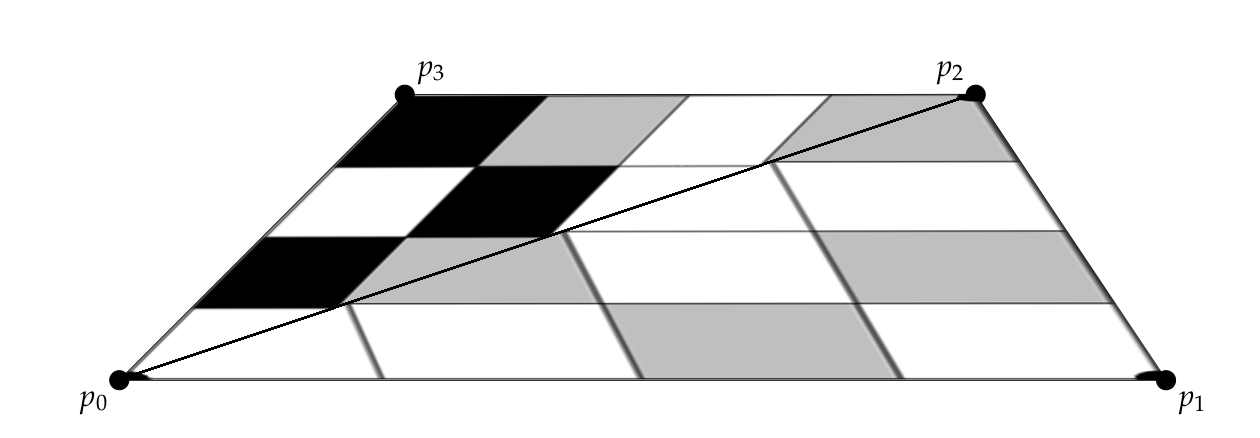
\includegraphics[scale = .2]{3d_2}\\

mit perspektivischer Korrektur: \\
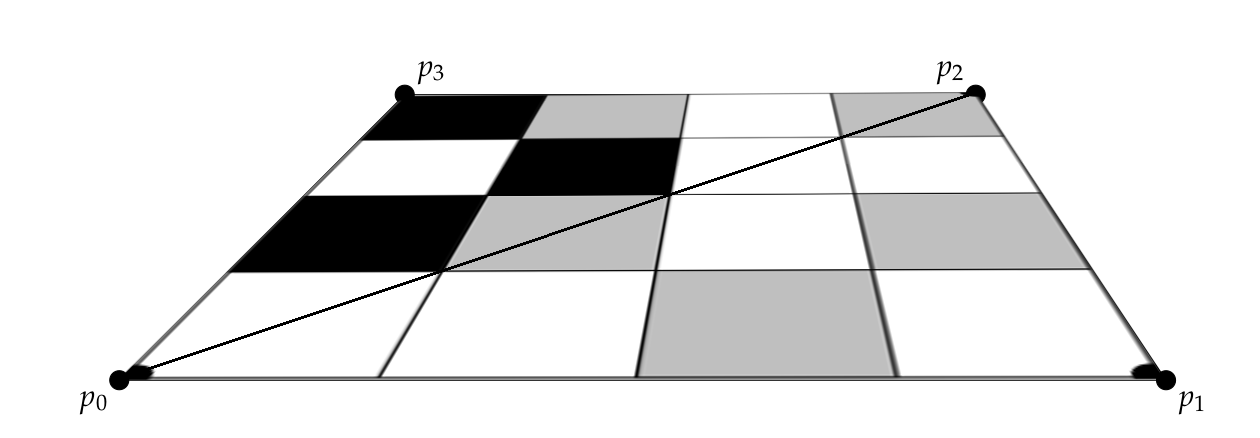
\includegraphics[scale= .2]{3d_1}

\end{document}
